\chapter{The main stages of the construction of a phylogenetic tree}
\section{Multiple sequences alignment}
To show the novelty of my work, at first need to 
understand what was researched previously.

Same stages of the actions are used to construct a phylogenetic tree in many methods.
They can be divided in three main actions.

\subsection{Stage 1: Align sequences} \label{phase1}

\begin{algorithm}[H]
\KwData{Given $n$ unaligned sequences\;}
\KwResult{$n$ aligned sequences\;}
\eIf{All sequnces have same length}{
	go to next phase\;
}
{
	Align all sequences\;
}
\end{algorithm}


Alignment methods vary in type of data \cite{rporter} (DNA, RNA, or amino-acid)
they can handle, and also, to some extent, the objectives of the alignment method \cite{tandy}.
Thus, some methods are designed exclusively for proteins, some exclusively
for RNAs, but many alignment methods can analyze both protein and nucleotide
datasets. We refer to methods that can analyze all types of molecular sequences as
``generic'' methods.

Sequence alignment is a way of arranging sequences of DNA, RNA, or 
proteins in order to distinguish regions of similarity. A multiple sequence 
alignment (MSA) is a sequence alignment of three or more biological sequences 
such as protein, DNA, or RNA. Typically it is implied that the set of sequences 
share an evolutionary relationship, which means they are all descendents from a 
common ancestor. These regions may correspond to functional, structural, or 
evolutionary relationships between the sequences. Alignments can reflect a degree 
of evolutionary change between sequences that are descendants from a common 
ancestor. There is a relationship between phylogenies and sequence alignments.

To find the globally optimum alignment, a dynamic programming technique 
can be used if one uses a parsimony approach and a particular scoring scheme. 
There is no universally agreed upon scoring scheme. This approach is 
computationally expensive and impractical since it has been shown to be a NP-complete 
problem. Instead, heuristics are commonly used to perform a multiple 
sequence alignment. This research focused on studying one heuristic approach 
called progressive alignment. One popular program that employs a progressive 
alignment method is ClustalW \footnote{ClustalW is a popular 
program used for multiple sequence alignment and for preparing phylogenetic trees}. 
Perform a multiple sequence alignment can be broken down into three major steps.
\nocite{clustalwsite}

\begin{description}
\item[FIRST], all pairs of sequences are aligned separately and then a distance 
matrix is calculated giving the divergence of each pair of sequences. A full 
dynamic programming alignment is calculated for each pair using two gap 
penalties, one for opening a gap and another for extending a gap. The score in the 
distance matrix is computed by taking the number of identities in the best 
alignment divided by the number of residues compared excluding gap positions. 
Then that number is multiplied by 100 and subtracted from 1.0 to give a value 
between 0 and 1.0.
\item[SECOND], a guide tree is calculated which will be used to guide the final 
multiple alignment process. This tree is calculated by using the distance matrix 
from the first step and a Neighbor-Joining clustering algorithm. Weights are also 
assigned to each sequence depending on their distance from the root of the tree. By 
contrast, in the original Clustal progressive alignment algorithm, all sequences 
would be equally weighted. 
\item[THIRTD], the sequences are progressively aligned according to the branching 
order in the guide tree. To do this a series of pairwise alignments are used to align 
larger and larger groups of sequences. First, proceed from the tips of the rooted 
tree towards the root. At each alignment a full dynamic programming algorithm is 
used with penalties for opening and extending gaps. Each step aligns two existing 
alignments or sequences. Gaps that are present in the older alignments stay in 
place. When all the sequences have been considered a final alignment is produced. 
That final alignment can then be used to construct a phylogenetic tree for those 
species. 
\item[Disadvantages:] One disadvantage of a progressive alignment approach is that, once an 
alignment has been performed involving some of the species, this alignment is 
never reconsidered despite what other decisions are made for the remaining species. 
This can lead to inaccuracies in the final alignment.
\end{description}

\section{Building Distance Matrix to campare taxons}

\subsection{Stage 2: Building Distance Matrix} \label{phase2}
An important tool in distance-based methods in building phylogenetic 
tree is the use of distance matrix. An $m*n$ matrix is a collection 
of $nm$ real numbers, arranged in $m$ rows and $n$ columns.

\[
M = \begin{bmatrix}
	a_{1,1} & a_{1,2} & \cdots & a_{1,n} \\
  	a_{2,1} & a_{2,2} & \cdots & a_{2,n} \\
  	\vdots  & \vdots  & \ddots & \vdots  \\
  	a_{m,1} & a_{m,2} & \cdots & a_{m,n}
\end{bmatrix}
\]

Each number $a_{ij}$ in the matrix is called an $entry$ of the $matrix$. 
A matrix is said to be $symmetric$ if for any row and column 
$i,j, a_{ij} = a_{ji}$. The following examples show the 
symmetry and asymmetry of matrices.

In particular, if a matrix has the same number of rows 
and columns, $n*n$, it is often called a square matrix. 
Given a collection of n sequences, with distance $d$ defined 
between any pair of sequences, the following matrix

\[
M = \begin{bmatrix}
	a_{1,1} & a_{1,2} & \cdots & a_{1,n} \\
  	a_{2,1} & a_{2,2} & \cdots & a_{2,n} \\
  	\vdots  & \vdots  & \ddots & \vdots  \\
  	a_{n,1} & a_{n,2} & \cdots & a_{n,n}
\end{bmatrix}
\]

is call the distance matrix, where $d_{ij}$ is the distance 
between the $i$th and $j$th sequences.

One of chanllenges in using distance matrices with distance 
methods to build phylogenetic tree is the building of the matrix. 
The very necessary condition to make all the thory work is that 
the distance must satisfy metric property. That is, all the 
entries in the distance matrix representing distances between 
sequences must satisfy the triangulr inequality,
\[
d_{ik} \leq d_{ij} + d_{jk},
\]

for all $1 \leq i,j,k \leq n$. Unfortunately, many times 
it is not the case in practice. There are always some 
entries fail the inequality, if not all of them.

Our first algorithm is to correct any possible errors to 
make the matrix symmetric. Assuming that, upon detection 
of asymmetries, there is no way algorithm would know which 
one is the true correct data, it simply uses the average 
of the two values to substitute. The pseudo-code for the 
algorithm is given in the following. 


\begin{algorithm}[H]
\KwData{n is the number of nodes, i=1\;}
\KwResult{retrieve data matrix in a double string\;}
\While{i!=n}{
	j=2\;
	\If{d[ij]!=d[ji]}{
		 substitute d[ij] and d[ji] by (d[ij]+d[ji])/2\;
	}
	j=j+1\; 
	\If{j=n}
	{
		i=i+1\;
	}  
}
\SetAlgoRefName{}	
\caption{Symmetry Enforcing - Iteration}
\end{algorithm}

The complexity of the algorithm is linear since the matrix 
has $O(n^2)$ entries.

\subsection{Metric distance matrix}
Assume we now have a symmetric distance matrix, our next 
challenge is to enforce the metric property. Again, 
our assumption is that the algorithm would not know the 
true correct data, it simply uses the minimum value to make 
the distance metric. More specifically, for a node $A_n$, 
if the triangular inequality holds, then for any $j,k < i$, 
we must have

\[
d_{ik} \geq d_{ij} - d_{jk},
\]

Thus,

\[
d_{ik} \geq \max_{k<j}(d_{ij} - d_{jk}),
\]

is a necessary condition for the triangular inequality to be true. 
The pseudo-code for the algorithm is given in the following.

\begin{algorithm}[H]
\KwData{n is the number of nodes; i=3\;}
\KwResult{retrieve data matrix M[n] in a double string\;}
\While{i!=n+1}{
	j=2\;
	k=1\;
	\If{ d[ij]<d[jk]-d[ik]}{
		 substitute d[ij] by d[jk]-d[ik]\;
	}
	k=k+1\; 
	\If{k=j}
	{
		j=j+1\;
	} 
	\If{j=i}
	{
		i=i+1\;
	}  
}
\SetAlgoRefName{}	
\caption{Metricalization of distance matrix}
\end{algorithm}

The complexity of the algorithm will also be polynomial since

\[
\sum_i^n i*i(i+1) \cong O(n^4)
\]

Also, the correction process is heavily based on the earlier 
portion of the data than the later portion. Namely, if a 
distance matrix fails the triangular property only at the 
last node or so, the correction is very minimum. 
On the other hand, if it occurs at the first three 
(automatically true with only two nodes) nodes, then it 
might have impact on all the data follows.

% \subsubsection{Benchmark datasets}
% Many studies have
% evaluated MSA methods using biological data for which structurally informed alignments
% are available. The best known of these benchmark datasets is probably BAliBASE,
% but others are also used. The choice of benchmarks and how they are used
% has a large impact on the result of the evaluation, and so has been discussed in several
% papers.
% 
% From the perspective of phylogeny estimation, one of the
% most important of their observations is that structurally-defined benchmarks often omit
% the highly variable parts of the molecule, including introns. Thus, an alignment can be
% considered completely correct as a structural alignment if it aligns the conserved regions,
% even if it fails to correctly align the variable regions. The problem with this criterion (as
% they point out) is that the highly variable portions are often the sites that are of most use
% for phylogeny estimation, whereas sites that change slowly have little phylogenetic signal.
% 
% \subsubsection{Relative performance of MSA methods}
% While most studies have evaluated alignment methods in terms of standard criteria 
% (notably, SP and TC scores) on biological
% benchmarks, some studies have explored alignment estimation for phylogeny estimation
% purposes. As commented on earlier, many studies have shown that alignment estimation
% impacts phylogenetic estimation, and that alignment and tree error increase with the rate
% of evolution. Also, on very large datasets, due to computational limitations, only a few
% alignment methods can even be run (and typically not the most accurate ones), which
% results in increased alignment error. On the other hand, on large trees with rates of
% evolution that are sufficiently low, alignment estimation methods can differ substantially
% in terms of SP-score without impacting the accuracy of the phylogenetic tree estimated
% using the alignment. More generally, standard alignment metrics may be only poorly
% correlated with tree accuracy in some conditions.
% 
% \subsubsection{Progressive aligners, and the impact of guide trees}
% Many alignment methods
% use progressive alignment on a guide tree to estimate the alignment; thus the choice of the
% guide tree and its impact on alignment and phylogeny estimation is also of interest. 
% Nelesen studied the impact of the guide tree on alignment methods,
% and showed that improved phylogenetic accuracy can be obtained by first estimating a tree
% from the input using a good two-phase method (RAxML on a MAFFT alignment).
% They noted particular benefits in using Probcons with this guide tree, and called the
% resultant method ``Probtree''. Prank has also been observed to be very sensitive to guide
% trees, and to give improved results by the use of carefully computed guide trees
% (maximum likelihood on good alignments). Another study showed that even
% when the alignment score doesn't change, the alignment itself can change in important
% ways when guide trees are changed. Finally, Capela-Gutierrez and Gabaldon
% found that the placement of gaps in an alignment results from the choice of the guide tree,
% and hence the gaps are not phylogenetically informative. Based on these observations,
% Capela-Gutierrez and Gabaldon recommended that alignment estimation methods should
% use the true tree (if possible), or else use an iterative co-estimation method that infers
% both the tree and the alignment.
% 
% \subsubsection{Template-based methods}
% Some alignment methods use a very different type of
% algorithmic structure, which is referred to as being ``template-based''. Instead of
% using progressive alignment on a guide tree, these methods use models (either profiles,
% templates, or Hidden Markov Models) for the gene of interest, and align each sequence to
% the model in order to produce the final multiple sequence alignment, as follows. First, a
% relatively small set of sequences from the family is assembled, and an alignment estimated
% for the set. Then, some kind of model (e.g., a template or a Hidden Markov Model) is
% constructed from this ``seed'' alignment. This model can be relatively simple or quite
% complex, typically depending on whether the model provides structural information. Once
% the model is estimated, the remaining sequences are added to the growing alignment. The
% model is used to align each sequence to the seed alignment (which does not change during
% the process), and then inserted into the growing alignment. Since the remaining sequences
% are only compared to the seed alignment, homologies between the remaining sequences
% can only be inferred through their homologies to the seed alignment. Thus, the choice
% of sequences in the seed alignment and how it is estimated can have a big impact on
% the resultant alignment accuracy. By design, once the seed alignment and the model
% are computed, the running time scales linearly with the number of sequences, and the
% algorithm is trivially parallelizable. Thus, these methods, which we will refer to jointly as
% ``template-based methods'', can scale to very large datasets with hundreds of thousands
% of sequences.
% 
% There are several examples of methods that use this approach. Some of these methods use curated seed alignments based on
% structure and function of well-characterized proteins or rRNAs; for example, the protein
% alignment method by Neuwald and the rRNA sequence alignment method by Gardner 
% use curated alignments. Constraint-based methods, such as COBALT,
% 3DCoffee and PROMALS, similarly use external information like structure and
% function, but then use progressive alignment techniques (or other such methods) to 
% produce the final alignment. Clustal-Omega also has a version, called ``External Profile
% Alignment'', that uses external information (in the form of alignments) to improve the
% alignment step.
% 
% Finally, PAGAN is another member of this class of methods; however, it has
% some specific methodological differences to the others. First, unlike several of the others,
% it does not use external biological information (about structure, function, etc.) to define
% its seed alignment. Second, while the others tend to use either HMMs, profiles, or 
% templates as a model to define the alignment of the remaining sequences, PAGAN estimates
% a tree on its seed alignment, and estimates sequences for the internal nodes. These 
% sequences are then used to define the incorporation of the remaining sequences to the seed
% alignment. This technique is very similar to the technique used in PaPaRa, which
% was developed for the phylogenetic placement problem. Thus, PAGAN
% is one of the ``phylogeny-aware'' alignment methods, a technique that is atypical of these
% template-based methods, but shared by progressive aligners. PAGAN was compared to an
% HMM-based method (using HMMER on the reference alignment to build an HMM, and
% then using HMMALIGN to align the sequences to the HMM) on several datasets.
% The comparison showed that PAGAN had very good accuracy, better than HMMALIGN,
% under low rates of evolution, and that both methods had reduced accuracy under high
% rates of evolution. They also noted that PAGAN failed to align some sequences under
% model conditions with high rates of evolution, while HMMER aligned all sequences; 
% however, the sequences that both HMMER and PAGAN aligned were aligned more accurately
% using PAGAN.
% 
% \subsubsection{Methods that use divide-and-conquer on the taxon set}
% Some alignment methods use a divide-and-conquer strategy in which the 
% taxon set is divided into subsets
% (rather than the sites) in order to estimate the alignment; these include the 
% mega-phylogeny method developed by Smith, SAT'e, SATCHMO-JS,
% PROMALS, and the method by Neuwald. (The SAT'e and SATCHMO-JS 
% methods co-estimate alignments and trees, and so are not strictly speaking just alignment
% methods.) Neuwald's method is a bit of an outlier in this set, because the user provides
% the dataset decomposition, but we include it here for comparative purposes.
% 
% While the methods differ in some details, they use similar strategies to estimate 
% alignments. Most estimate an initial tree, and then use the tree to divide the dataset into
% subsets. The method to compute the initial trees differs, with SATCHMO-JS using a
% neighbor joining (NJ) tree on a MAFFT alignment, SAT'e using a maximum 
% likelihood tree on a MAFFT alignment, PROMALS using a UPGMA tree on $k$-mer distances,
% and mega-phylogeny using a reference tree and estimated alignment.
% 
% The subsequent division into subsets is performed in two ways. In the case of 
% mega-phylogeny, SATCHMO-JS, and PROMALS, the division into subsets is performed by
% breaking the starting tree into clades so as to limit the maximum dissimilarity between
% pairs of sequences in each set. In contrast, SAT'e-2 removes centroid edges from the
% unrooted tree, recursively, until each subset is small enough (below 200 sequences). Thus,
% the sets produced by the SAT'e-2 decomposition do not form clades in the tree, unlike the
% other decompositions. Furthermore, the sets produced by the SAT'e-2 decomposition are
% guaranteed to be small (at most 200 taxa) but are not constrained to have low pairwise
% dissimilarities between sequences.
% 
% Alignments are then produced on each subset, with PROMALS, SAT'e, and 
% mega-phylogeny estimating alignments on each subset, and SATCHMO-JS using the alignment
% induced on the subset by the initial MAFFT alignment.
% 
% These alignments are then merged together into an alignment on the full set, but the
% methods use different techniques. PROMALS and mega-phylogeny use template-based
% methods to merge the alignments together, while SATCHMO-JS and SAT'e use progressive
% alignment techniques. PROMALS also uses external knowledge about protein structure
% to guide the template-based merger of the alignments together. PROMALS, 
% SATCHMO-JS, and mega-phylogeny use sophisticated methods to merge subset-alignments, but SAT'e
% uses a very simple method (Muscle) to merge subset-alignments.
% 
% \subsubsection{Very large-scale alignment}
% When the datasets are very large, containing many
% thousands of sequences, only a few alignment estimation methods are able to run. As
% noted, the template-based methods (including PROMALS and mega-phylogeny) scale
% linearly with the number of taxa, and so can be used with very large datasets. SAT'e
% and SATCHMO-JS are not quite as scalable; however, SAT'e has been able to analyze
% nucleotide datasets with about 28,000 sequences. Other methods that have been shown to
% run on very large datasets include Clustal-Omega, MAFFT-PartTree, and 
% Kalign-2, but many methods fail to run on datasets with tens of thousands of sequences.
% Of these, Clustal-Omega is only designed for protein sequences, but MAFFT-PartTree
% and Kalign-2 can analyze both nucleotide and amino-acid sequences.
% 
% SAT'e is computationally limited by its use of progressive alignment and maximum
% likelihood method (RAxML or FastTree-2) in each iteration; both impact the 
% running time and - in the case of large numbers of long sequences - memory usage. However,
% although limited to datasets with perhaps only 30,000 sequences (or so), on fast-evolving
% datasets with 1000 or more sequences, SAT'e provides improvements in phylogenetic 
% accuracy relative to competing methods.

\section{Phylogenetic tree generation}

\subsection{Stage 3: Reconstructing phylogenetic tree}

Before proceeding to the construction of a phylogenetic tree, you should examine the 
existing models of gene sequences.

\subsection{Stochastic models of sequence evolution}
We begin with a description of the simplest stochastic models of DNA sequence 
evolution, and then discuss amino-acid sequence evolution models and codon evolution models.
The simplest models of DNA sequence evolution treat the sites within the sequences 
independently. Thus, a model of DNA sequence evolution must describe the probability
distribution of the four states, A, C, T, G, at the root, the evolution of a random site (i.e.,
position within the DNA sequence) and how the evolution differs across the sites. 
Typically the probability distribution at the root is uniform (so that all sequences of a fixed
length are equally likely). The evolution of a single site is modeled through the use of
``stochastic substitution matrices'', $4 x 4$ matrices (one for each tree edge) in which every
row sums to 1. A stochastic model of how a single site evolves can thus have up to 12 free
parameters. The simplest such model is the Jukes-Cantor model, with one free parameter,
and the most complex is the General Markov model, with all 12 parameters:

\begin{defn}
The General Markov (GM) model of single-site evolution is defined as follows.

\begin{enumerate}
	\item The nucleotide in a random site at the root is drawn from a known distribution, in
which each nucleotide has positive probability.
	\item The probability of each site substitution on an edge $e$ of the tree is given by a $4 x 4$
stochastic substitution matrix $M(e)$ in which $det(M(e))$ is not $0$, $1$, or $-1$.	
\end{enumerate}
\end{defn}

This model is generally used in a context where all sites evolve identically and 
indpendently (the i.i.d. assumption), with rates of evolution drawn typically drawn from a
gamma distribution. (Note that the distribution of the rates-across-sites has an impact
on phylogeny estimation and dating, as discussed by Evans and Warnow.) In what
follows, we will address the simplest version of the GM model so that all sites have the
same rate of evolution.

We denote a model tree in the GM model as a pair, ($T, {M(e): e \in E(T)}$), or more
simply as $(T, M)$. For each edge $e \in E(T)$, we define the length of the edge $\lambda(e)$ to
be - $log |det(M(e))|$. This allows us to define the matrix of leaf-to-leaf distances, ${\lambda_{ij}}$,
where $\lambda_{ij} = \sum_{e \in P_{ij}}$
$\lambda(e)$, and where $P_{ij}$ is the path in $T$ between leaves $i$ and $j$. A
matrix defined by path distances in a tree with edge weights is called ``additive'', and it
is a well-known fact that given any additive matrix, it is easy to recover the underlying
leaf-labelled tree T for that matrix in polynomial time.

This general model of site evolution subsumes the great majority of other models
examined in the phylogenetic literature, including the popular General Time Reversible
(GTR) model, which requires only that $M(e) = M(e')$
for all edges $e$ and $e'$. 
Further constraints on the matrix $M(e)$ produce the Hasegawa-Kishino-Yang (HKY) model,
the Kimura 2-parameter model (K2P), the Kimura 3-ST model (K3ST), the Jukes-Cantor
model (JC), etc. These models are all special cases of the General Markov model, because
they place restrictions on the form of the stochastic substitution matrices. The standard
model used for nucleotide phylogeny estimation is GTR+gamma, i.e., the General Time
Reversible (GTR) model of site substitution, equipped with a gamma distribution of rates
across sites.

\subsection{Protein models}
Just as with DNA sequence evolution models, there are Markov
models of evolution for amino-acid sequences, and also for coding DNA sequences. These
models are described in the same way - a substitution matrix that governs the tree,
and then branch lengths. While the GTR model can be extended to amino-acids (to
produce a $20x20$ matrix) or to codon-based models (to produce a $64x64$ matrix), both
of which must be estimated from the data, in practice these models use fixed matrices,
each of which was estimated from external biological data. The most well known protein
model is the Dayhoff model, but improved models have been developed in recent
years. Similarly, codon-based models have also been based on fixed $64x64$
matrices. In practice, the selection of a protein model for a given dataset
is often done using a statistical test, such as ProtTest, and then fixed. In the
subsequent tree estimation performed under that model, only the tree and its branch
lengths need to be estimated.

\subsection{Phylogeny Estimation Methods}
There are many different phylogeny estimation methods, too numerous to mention here.
However, the major ones can be classified into the following types:

\begin{itemize}
	\item distance-based methods, which first compute a pairwise distance matrix (usually
based on a statistical model) and then compute the tree from the matrix,
	\item maximum parsimony and its variants, which seek a tree with a total minimum
number of changes (as defined by edit distances between sequences at the endpoints
on the edges of the tree),
	\item maximum likelihood, which seeks the model tree that optimizes likelihood
under the given Markov model, and
	\item Bayesian MCMC methods, which return a distribution on trees rather than a single
tree, and also use likelihood to evaluate a model tree.	
\end{itemize}

\subsection{Statistical Performance Criteria}
We discuss three concepts here: \textit{identifiability, statistical consistency, 
and sequence length requirements}.


\textbf{Identifiability:} A statistical model or one of its parameters is said to be 
``identifiable'' if it is uniquely determined by the probability distribution 
defined by the model. Thus, in the context of phylogeny estimation, the 
unrooted model tree topology is identifiable if it is determined by the 
probability distribution (defined by the model tree, which includes the 
numeric parameters) on the patterns of nucleotides at the leaves of the tree. 
In the case of nucleotide models, the state at each leaf can be A,C,T, or G, 
and so there are $4^n$ possible patterns in a tree with n leaves 
(similarly, there are $20^n$ possible patterns for amino-acid models). 
It is well known that the unrooted tree topology is identifiable under 
the General Markov model, and recent work has extended this to 
other models.

\textbf{Statistical Consistency:} We say that a method $\Phi$ is ``statistically consistent'' 
for estimating the topology of the model tree $(T,\theta )$ if the trees estimated 
by $\Phi$ converges to the unrooted version of $T$ (denoted by $T^u$) as the number 
of sites increases. (Note that under this definition, we are not concerned 
with estimating the numeric parameters.) Equivalently, for all $\varepsilon > 0$ there 
is a sequence length $K$ so that if a set $S$ of sequences of length $k \geq K$ are 
generated by $(T,\theta)$, then the probability that $\Phi(S) = T^u$ is at least $1-\varepsilon$. 
We say that a method is statistically consistent under the GM model if 
it is statistically consistent for all model trees in the GM model. 
Similarly, we say a method is statistically consistent under the GTR 
model if it is statistically consistent under all model trees in the GTR model. 

Many phylogenetic methods are statistically consistent under the GM model, 
and hence also under its submodels (e.g., the GTR model). For example, 
maximum likelihood, neighbor joining (and other distance-based methods) 
for properly computed pairwise ``distances'', and Bayesian MCMC methods, 
are all statistically consistent. Onthe other hand, maximum parsimony and 
maximum compatibility are not statistically consistent under the GM 
model. In addition, it is well known that maximum likelihood can be 
inconsistent if the generative model is different from the model 
assumed by maximum likelihood, but maximum likelihood can even be 
inconsistent when its assumptions match the generative model, 
if the generative model is too complex! For example, 
Tuffey and Steel showed that maximum likelihood is equivalent 
to maximum parsimony under a very general ``no-common-mechanism'' model, 
and so is inconsistent under this model. In this case, the model 
itself is not identifiable, and this is why maximum likelihood 
is not consistent. However, there are identifiable models for 
which ML is not consistent, as observed by Steel.

\textbf{Sequence length requirement:} Clearly, statistical consistency 
under a model is a desirable property. However, statistical consistency 
does not address how well a method will work on finite data. 
Here, we address the ``sequence length requirement'' of a phylogeny 
estimation method $\Phi$, which is the number of sites that $\Phi$ needs 
to return the (unrooted version of the) true tree with 
probability at least $1 - \epsilon$ given sequences that evolve 
down a given model tree $(T,\theta)$. Clearly, the number of 
sites that suffces for accuracy with probability at 
least $1 - \epsilon$ will depend on $\Phi$ and $\epsilon$, but it also 
depends on both $T$ and $\theta$. 

We describe this concept in terms of the Jukes-Cantor model, 
since this is the simplest of the DNA sequence evolution models, 
and the ideas are easiest to understand for this model. However, 
the same concepts can be applied to the more general models, and 
the theoretical results that have been established regarding sequence 
length requirements extend to the GM (General Markov) model, which 
contains the GTR model and all its submodels.

In the Jukes-Cantor (JC) model, all substitutions are equally likely, 
and all nucleotides have equal probability for the root state. 
Thus, a Jukes-Cantor model tree is completely defined by the rooted 
tree $T$ and the branch lengths $\lambda(e)$, where $\lambda(e)$ is 
the expected number of changes for a random site on the edge $e$. 
It is intuitively obvious that as the minimum branch length 
shrinks, the number of sites that are needed to reconstruct the 
tree will grow, since a branch on which no changes occur 
cannot be recovered with high probability (the branch will appear 
in an estimated tree with probability at most one-third, 
since at best it can result from a random resolution of a 
node of degree at least 4). It is also intuitively obvious 
that as the maximum branch length increases, the number of 
sites that are needed will increase, since the two sides 
of the long branch will seem random with respect to each other. 
Thus, the sequence length requirement for a given method to be 
accurate with probability at least $1 - \epsilon$ will be 
impacted by the shortest branch length f and the longest 
branch length $g$. It is also intuitively obvious that the 
sequence length requirement will depend on the number of 
taxa in the tree.  

Expressing the sequence length requirement for the 
method $\Phi$ as a function of these parameters ($f,g,n$ and $\epsilon$) 
enables a different - and finer - evaluation of the method's performance 
guarantees under the statistical model. Hence, we consider $f,g$, and $\epsilon$ 
as fixed but arbitrary, and we let JCf,g denote all Jukes-Cantor model 
trees with $0 < f \leq \lambda(e) \leq g < \infty$ for all edges $e$. 
This lets us bound the sequence length requirement of a method as a 
function only of $n$, the number of leaves in the tree. 

The definition of ``absolute fast convergence'' under the Jukes-Cantor 
model is formu- lated as an upper bound on the sequence length requirement, 
as follows:

\begin{defn}
A phylogenetic reconstruction method $\Phi$ is absolute fast-converging (afc) 
for the Jukes-Cantor (JC) model if, for all positive $f,g$, and $\varepsilon$, 
there is a polynomial $p(n)$ such that, for all $(T,\theta)$ in $JC_{f,g}$, 
on set $S$ of $n$ sequences of length at least $p(n)$ generated on $T$, 
we have $Pr[\Phi(S) = T^u] > 1 - \varepsilon$.
\end{defn}

Note also that this statement only refers to the estimation of the unrooted 
tree topology $T^u$ and not the numeric parameters $\Phi$. Also, note that 
the method $\Phi$ operates without any knowledge of parameters $f$ or $g$-or 
indeed any function of $f$ and $g$. Thus, although the polynomial $p$ 
depends upon both $f$ and $g$, the method itself will not. Finally, this 
is an upper bound on the sequence length requirement, and the actual 
sequence length requirement could be much lower. 

The function $p(n)$ can be replaced by a function $f(n)$ that is not 
polynomial to provide an upper bound on the sequence length requirement 
for methods that are not proven to be absolute fast converging. 

\subsection{Empirical Performance}
So far, these discussions have focused on theoretical guarantees under a model, 
and have addressed whether a method will converge to the true tree given 
long enough sequences (i.e., statistical consistency), and if so, then 
how long the sequences need to be (sequence length requirements). However, 
these issues are purely theoretical, and do not address how accurate the 
trees estimated by methods are in practice (i.e., on data). In addition, 
the computational performance (time and memory usage) of phylogeny estimation 
methods is also important, since a method that is highly accurate but will 
use several years of compute time will not generally be useful in most analyses. 

Phylogenetic tree accuracy can be computed in various ways, and there are 
substantive debates on the ``right'' way to calculate accuracy; however, 
although disputed, the Robinson-Foulds (RF) distance, also called the 
``bipartition distance'', is the most commonly used metric on phylogenetic trees. 
We describe this metric here. 

Given a phylogenetic tree $T$ on $n$ taxa, each edge can be associated 
with the bipartition it induces on the leaf set; hence, the tree 
itself can be identified with the set of leaf- bipartitions defined 
by the edges in the tree. Therefore, two trees on the same set 
of taxa can be compared with respect to their bipartition sets. 
The RF distance between two trees is the size of the symmetric difference 
of these two sets, i.e., it is the number of bipartitions that are in one 
tree's dataset but not both. This number can be divided by $2(n - 3)$ 
(where n is the number of taxa) to obtain the ``RF rate''. In the context 
of evaluating phylogeny estimation methods, the RF distance is sometimes 
divided into false negatives and false positives, where the false 
negatives (also called ``missing branches'') are branches in the 
true tree that are not present in the estimated tree, and the 
false positives are the branches in the estimated tree that are not 
present in the true tree. This distinction between false positives 
and false negatives enables a more detailed comparison between trees 
that are not binary.

Many studies have evaluated phylogeny estimation methods on simulated 
data, varying the rate of evolution, the branch lengths, the number 
of sites, etc. These studies have been enormously informative about 
the differences between methods, and have helped biologists make 
informed decisions regarding methods for their phylogenetic analyses. 
Some of the early simulation studies explored performance on very 
small trees, including the fairly exhaustive study by Huelsenbeck 
and Hillis on 4-leaf trees, but studies since then have explored 
larger datasets and more complex questions. For example, studies 
have explored the impact of taxon sampling on phylogenetic 
inference, the impact of missing data on phylogenetic inference, 
and the number of sites needed for accuracy with high probability. 
In fact, simulation studies have become, perhaps, the main way to 
explore phylogenetic estimation. 

\subsubsection{Distance-based methods} \label{methods}
Distance-based methods operate by first computing a matrix of 
distances (typically using a statistically defined technique, 
to correct for unseen changes) between every pair of sequences, 
and then construct the tree based on this matrix. Most, but not all, 
distance-based methods are statistically consistent, and so will 
be correct with high probability, given long enough sequences. 
In general, distance-based methods are polynomial time, and so 
have been popular for large-scale phylogeny estimation. 
While the best known distance-based method is probably neighbor 
joining, there are many others, and many are faster and/or 
more accurate. 

One of the interesting properties about distance-based 
methods is that although they are typically guaranteed 
to be statistically consistent, not all distance-based 
methods have good empirical performance! A prime example 
of this lesson is the Naive Quartet Method, a method that 
estimates a tree for every set of four leaves using the 
Four-Point Method (a statistically-consistent distance method) 
and then returns the tree that is consistent with all the 
quartets if it exists. It is easy to show that the Naive 
Quartet Method runs in polynomial time and is statistically 
consistent under the General Markov model; however, because 
it requires that every quartet be accurately estimated, 
it has terrible empirical performance! Thus, while 
statistical consistency is desirable, in many cases statistically 
inconsistent methods can outperform consistent ones.

\subsubsection{Maximum parsimony}
Maximum parsimony (MP) is NP-hard, and so the methods for 
MP use heuristics (most without any performance guarantees). 
The most efficient and accurate maximum parsimony software 
for very large datasets is probably TNT, but PAUP* is also 
popular and effective on datasets that are not extremely large. 
TNT is a particularly effective parsimony heuristic for 
large trees, and has been able to analyze a multi-marker 
sequence dataset with more than 73,000 sequences.

\subsubsection{Maximum likelihood}
Maximum likelihood (ML) is also NP-hard, and so attempts to 
solve ML are also made using heuristics. While the heuristics 
for MP used to be computationally more efficient than the 
heuristics for ML, the current set of methods for ML are 
quite effective at ``solving'' large datasets. (Here the 
quotes indicate that there is no guarantee, but reasonably 
good results do seem to be obtained using the current best software.)

The leading methods for large-scale ML estimation under the 
GTR+Gamma model include RAxML, FastTree-2, PhyML, and GARLI. 
Of these four methods, RAxML is clearly the most frequently 
used ML method, in part because of its excellent parallel 
implementations. However, a recent study showed that trees 
estimated by FastTree-2 were almost as accurate as those 
estimated by RAxML, and that FastTree-2 finished in a 
fraction of the time; for example, FastTree-2 was able to 
analyze an alignment with almost 28,000 rRNA sequences 
in about 5 hours, but RAxML took much longer. 
Furthermore, FastTree-2 has been used to analyze larger 
datasets (ones with more sequences) than RAxML: the 
largest dataset published with a RAxML analysis 
had 55,000 nucleotide sequences, but FastTree has 
analyzed larger datasets. For example, FastTree-2 
has analyzed a dataset with more than 1 million nucleotide 
sequences, and another with 330,556 sequences. 
The reported running time for these analyses are 203 
hours for the million-taxon dataset, and 13 hours 
(with 4 threads) for the 330K- taxon dataset 
\footnote{Morgan Price, personal communication, May 1, 2013.}. 
By comparison, the RAxML analysis of 55,000 nucleotide 
sequences took between 100,000 and 300,000 CPU hours
\footnote{Alexis Stamatakis, personal communication, May 1, 2013.}. 
The difference in running time is substantial, but we 
should note two things: the RAxML analysis was a 
multi-marker analysis, and so the sequences were much 
longer (which impacts running time), and because RAxML 
is highly parallelized, the impact of the increased running 
time is not as significant (if one has enough processors). 
Nevertheless, for maximum likelihood analysis of alignments 
with large numbers of sequences, FastTree-2 provides 
distinct speed advantages over RAxML.  

There are a few important limitations for FastTree-2, 
compared to RAxML. First, FastTree-2 obtains its speed by 
somewhat reducing the accuracy of the search; thus, the 
trees returned by FastTree-2 may not produce maximum 
likelihood scores that are quite as good as those produced 
by RAxML. Second, FastTree-2 doesn't handle very long 
alignments with hundreds of thousands of sites very well, 
while RAxML has a new implementation that is designed 
specifically for long alignments. Third, FastTree-2 has a 
smaller set of models for amino-acid analyses than RAxML. 
Therefore, in some cases (e.g., for wide alignments, 
and perhaps for amino-acid alignments), RAxML may 
be the preferred method. 

However, the ML methods discussed above estimate trees under 
the GTR+Gamma model, which has simplifying assumptions that 
are known to be violated in biological data. 
The nhPhyml method is a maximum likelihood method for 
estimating trees under the non-stationary, non-homogeneous 
model of Galtier and Guoy, and hence provides an 
analytical advantage in that it can be robust to some 
violations of the GTR+Gamma model assumptions. However, 
nhPhyml seems to be able to give reliably good analyses 
only on relatively small datasets (i.e., with at most a 
few hundred sequences, or fewer sequences if they are very long). 
The explanation is computational - it uses NNI 
(nearest neighbor interchanges, see below) to search treespace, 
but NNI is relatively ineffective, which means that it is 
likely to get stuck in local optima. This is unfortunate, 
since large datasets spanning substantial evolutionary 
distances are most likely to exhibit an increased incidence 
in model violations. Therefore, highly accurate phylogeny 
estimation of large datasets may require the use of new 
methods that are based upon more realistic, and more general, 
models of sequence evolution.

% \subsubsection{Bayesian MCMC methods}
% Bayesian methods are similar to maximum likelihood methods 
% in that the likelihood of a model tree with respect to the 
% input sequence alignment is computed during the analysis; 
% the main difference is that maximum likelihood selects the 
% model tree (both topology and numeric parameters) that 
% optimizes the likelihood, while a Bayesian method outputs a 
% distribution on trees. However, once the distribution is 
% computed, it can be used to compute a single point estimate 
% of the true tree using various techniques (e.g., a consensus 
% tree can be computed, or the model tree topology with the 
% maximum total probability can be returned).
% 
% The standard technique used to estimate this distribution 
% is a random walk through the model tree space, and the 
% distribution is produced after the walk has converged to 
% the stationary distribution.
% 
% There are many different Bayesian methods (e.g., MrBayes, BEAST, 
% PhyloBayes, p4, and BayesPhylogenies), differing in terms 
% of the techniques used to perform the random walk, and 
% the model under which the likelihood is computed; however, 
% MrBayes is the most popular of the methods. Bayesian 
% methods provide theoretical advantages compared to 
% maximum likelihood methods. However, the proper use of a 
% Bayesian MCMC method requires that it run to convergence, 
% and this can take a very long time on large datasets. 
% Thus, from a purely empirical stand- point, Bayesian 
% methods do not yet have the scalability of the best 
% maximum likelihood methods, and they are generally 
% not used on very large datasets.

\subsection{Comparisons between methods} \cite{hall}
Simulation studies have shown some interesting 
differences between methods. For example, the 
comparison between neighbor joining and maximum 
parsimony reveals that the relative performance may 
depend on the number of taxa and the rate of evolution, 
with maximum parsimony sometimes performing better 
on large trees with high rates of evolution, even 
though the reverse generally holds for smaller trees.  

\begin{figure}[t] 
  \center
  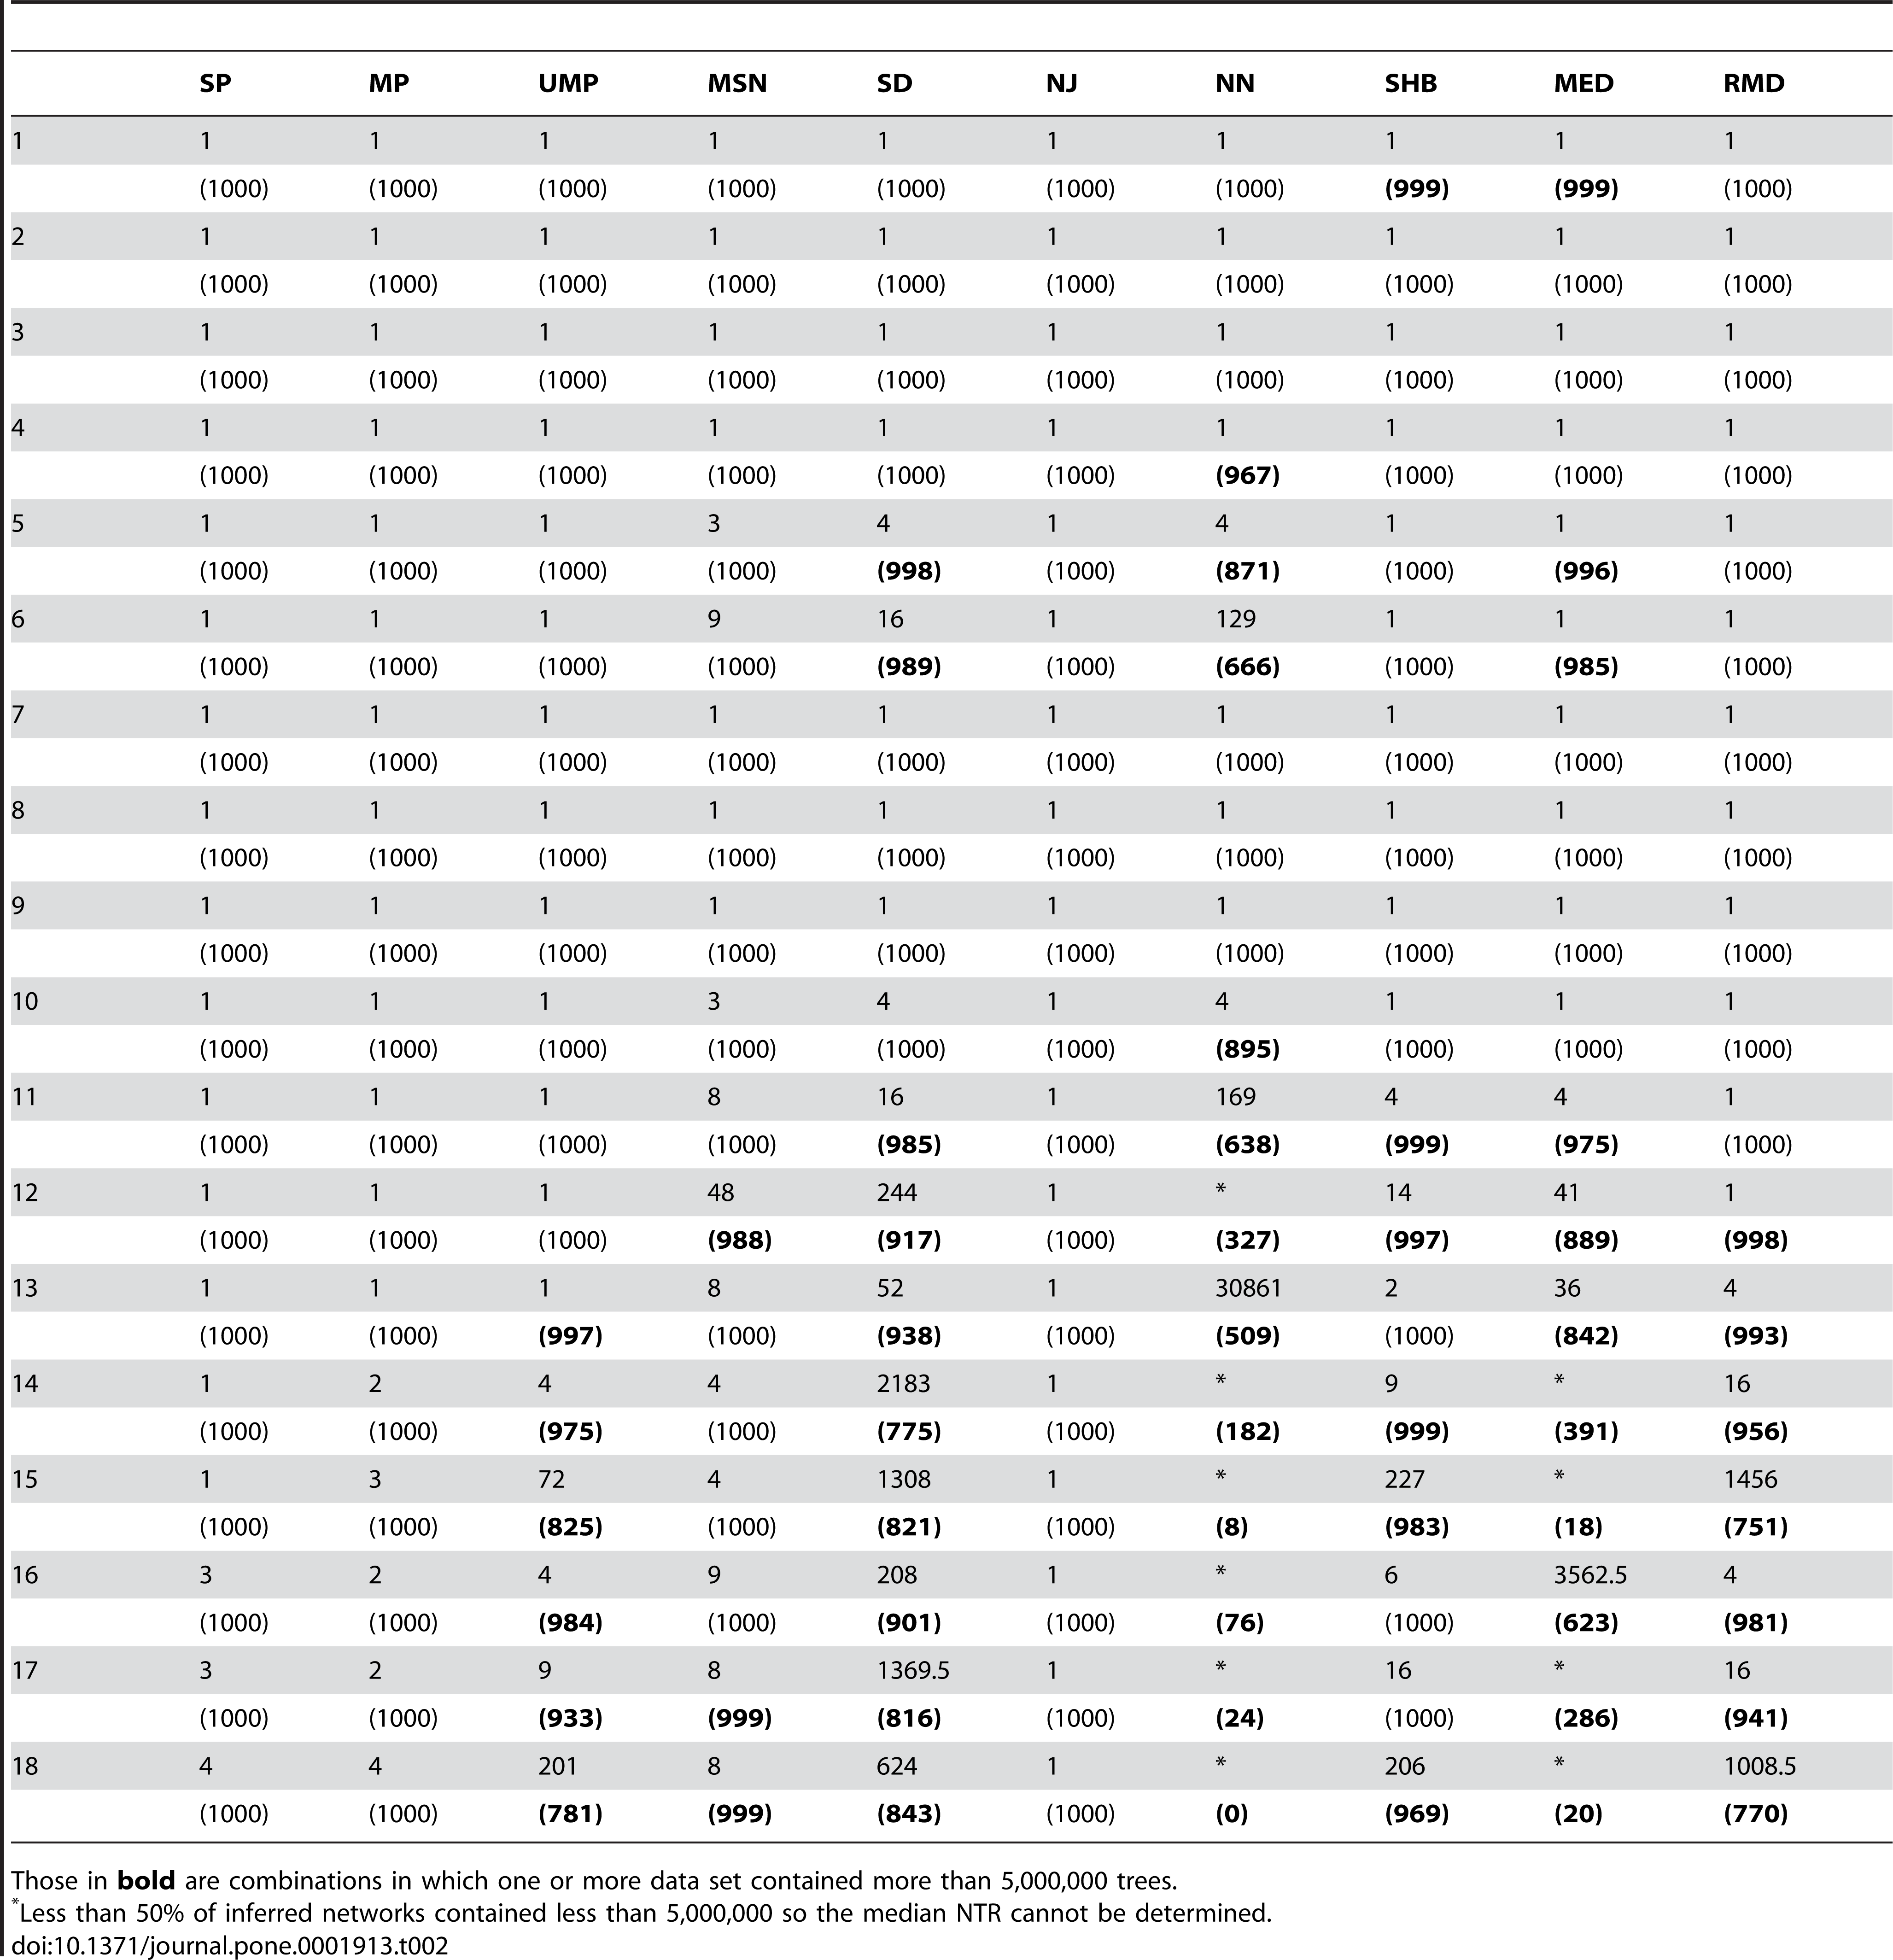
\includegraphics[width=1\textwidth]{comparison}
  \caption[w]{A comparison of phylogenetic methods \cite{comparison}} 
  \label{img:comparison}  
\end{figure}

More generally, most simulation studies have shown 
that maximum likelihood and Bayesian methods 
(when they can be run properly) outperform maximum 
parsimony and distance-based methods in many 
biologically realistic conditions 
(see Wang et al. for one such study). \cite{simmons}

\subsection{Heuristics for exploring treespace}
Since both maximum likelihood and maximum parsimony 
are NP-hard, methods for ``solving'' these problems 
use heuristics to explore the space of different tree 
topologies. These heuristics differ by the techniques 
they use to score a candidate tree (with the best 
ones typically using information from previous 
trees that have already been scored), and how 
they move within treespace. 
 
% \section{Methods of research}

\addcontentsline{toc}{section}{\numberline{}Conclusion for Chapter 2}
\section*{Conclusion for Chapter 2}

- Alignment methods vary in type of data \cite{rporter} (DNA, RNA, or aminoacid)
they can handle

- There are three main stages to reconstruct phylogenetic tree:
sequences aligment, calculate distance matrix, reconstruction tree.

- Neighbor joining is the simplest methods for reconstructing
phylogenetic trees.

- Maximum parsimony sometimes performing better 
on large trees with high rates of evolution, even 
though the reverse generally holds for smaller trees. 
 

\newpage